\documentclass[answers]{exam}
\usepackage{graphicx} % Required for inserting images
\usepackage[margin=1in]{geometry}
\usepackage{amsmath}
\usepackage{amssymb} % for \square
\usepackage{amsthm}
\usepackage{float}
\usepackage{tikz}
\usetikzlibrary{calc}

\usepackage[en-US,showdow]{datetime2}

\newcommand{\ds}{\displaystyle}
\newcommand{\Z}{\mathbb{Z}}
\newcommand{\arc}{\rightarrow}
\newcommand{\R}{\mathbb{R}}
\newcommand{\N}{\mathbb{N}}
\newcommand{\Q}{\mathbb{Q}}

\newcommand{\stirling}[2]{\genfrac{\{}{\}}{0pt}{}{#1}{#2}}

\usepackage{mathtools}
\def\multiset#1#2{\ensuremath{\left(\kern-.3em\left(\genfrac{}{}{0pt}{}{#1}{#2}\right)\kern-.3em\right)}}

\newtheorem{theorem}{Theorem}
\newtheorem{definition}{Definition}

\title{Midterm Adventure}
\author{Athor \# 1 \\
Author \# 2 \\
Author \# 3 }
\date{}

\begin{document}
\maketitle



	\section*{Rules of Engagement}
	
	You may discuss the problems below with anyone in the following set of people:
	\begin{eqnarray*}P &=& \{\mbox{Anyone currently enrolled in MATH 3310}, \\ 		&& \mbox{Kaylee Bodily, Caroline Torman, Erin Pitts, Brent Thomas}\}.\end{eqnarray*}
	
    The documentation of your adventure should be created by teams of at most 4 and is to be submitted by \DTMdate{2026-03-06} as a PDF via Canvas (the way we've done all semester). One submission per team.\\
        
    No outside resources are to be used on this experience.
	Try to get through this with your brain and the brains of your team (if you choose to be part of one). \\
	
	
	\section{The Adventure Begins} 
	
	\subsection*{Sneaking into Hogsmeade}
	\qformat{\textbf{Sub-Adventure \thesection.\thequestion }\hfill}
	\begin{questions}
		\question 
		
		Argus Filch and Severus Snape are playing a game in which they try to destroy all secret passages between Hogwarts, Hogsmeade, and the Shrieking Shack. Argus and Severus take turns destroying passages. On their turn, they select a location and destroy any positive number of passages to the other two locations. The winner of the game is the player who is able to destroy all the remaining passages on their turn.

	As an example, suppose there are 2 passages between the Shrieking Shack and Hogwarts, 1 passage between Hogwarts and Hogsmeade, and 3 passages between the Shrieking Shack and Hogsmeade.
		
		\begin{center}
			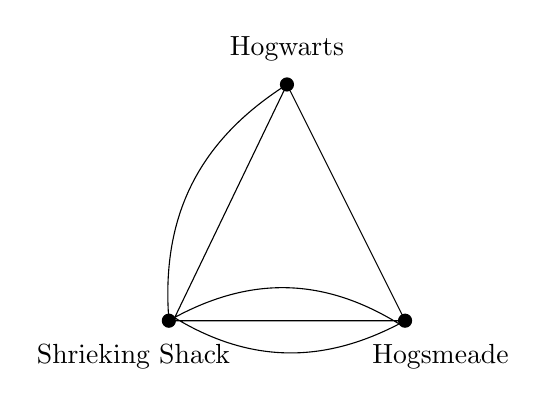
\begin{tikzpicture}[scale = 1.5]
				\tikzset{vertex/.style = {shape=circle,fill = black, draw, scale = 0.50}}
				
				%\node[] (label_d0) at (-4,0) {$K_1$};
				
				\node[vertex] (A) at (0,0) {};
				\node[] (label_A) at (-0.3,-0.3) {Shrieking Shack};
				\node[vertex] (B) at (2,0) {};
				\node[] (label_B) at (2.3,-0.3) {Hogsmeade};
				\node[vertex] (C) at (1,2) {};
				\node[] (label_C) at (1,2.3) {Hogwarts};
				
				\draw[] (A) to (B) to (C) to [bend right] (A) to [bend right] (B) 
				to [bend right] (A) to (C);
				
			\end{tikzpicture}
		\end{center}
		

		Suppose, in general, there are $x$ passages between the Shrieking Shack and Hogwarts, $y$ passages between Hogwarts and Hogsmeade, and $z$ passages between the Shrieking Shack and Hogsmeade.

		\emph{Determine, with proof, the values of $x,y,z$ for which Severus Snape (the first player) can always win if a particular strategy is employed for each move.}\\
		
		\begin{solution}
			
		\end{solution}
		
		
		\fullwidth{\subsection*{Dots and Boxes}}
		
		\question
		
		Two players, Link and Zelda, alternately select an \emph{edge} (a line segment connecting two dots) on the grid graph shown 
		below and color it red.
		The loser of the game is the player who is forced to select an edge that creates
		a red $C_4$ --- a red square on $4$ vertices.\\
		
		\begin{center}
			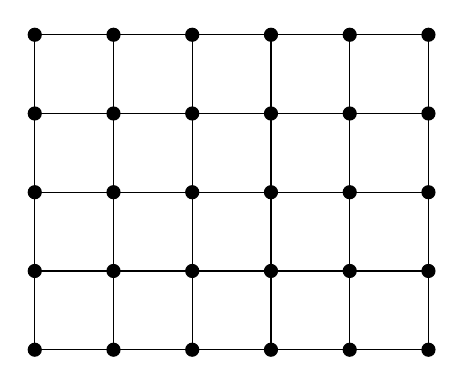
\begin{tikzpicture}[scale = 1]
				\tikzset{vertex/.style = {shape=circle,fill = black, draw, scale = 0.50}}
				\foreach \x in {0,1,2,3,4,5}{
					\foreach \y in {0,1,2,3,4}{
						\node[vertex] (\x\y) at (\x,\y) {};
				}}
				\draw (0,0) grid (5,4);
			\end{tikzpicture}
		\end{center}
		
		
		\noindent \emph{Confirm or deny, with proof, whether Zelda (the first player) can always 
			win if she employs a particular strategy for each move.}
		
		\begin{solution}
			
		\end{solution}
		
		
	\end{questions}
	
	\section{Prime Time}
		\qformat{\textbf{Sub-Adventure \thesection.\thequestion }\hfill}
		\begin{questions}	
			\question Prove or disprove whether you can order the years $2011, \dots, 2026$ so that the resulting $64$-digit number is prime.

			\begin{solution}
		\subsection*{Claim}
		It is not possible to order the years 2011, 2012, \dots, 2026 to form a 64-digit number that is prime. 

		\subsection*{Proof}
		We shall prove this by proving that any such 64-digit number formed by concatenating the years 2011 to 2026 is divisible by 11, and thus composite (Composite means not Prime).

		First we will start by refering to a few things from our notes. According to Theorem 2, part 6, we know that an integer $X$ is divisible by 11 if the alternating sum of its digits, $\sum_{i=0}^{n}(-1)^{i}d_{i}$, is divisible by 11.

		So we will concatinate each year, which which will give us our 64-digit number because we have 16 years and each year has 4 digits. Because each years is just 4 digits, which is an even number of digits, the alternating sum of each year will always be the same, (For example 2011 will always be $1 - 1 + 0 - 2$ no matter where we place it in the 64 digit number). 


		We calculate the individual alternating sums ($d_0 - d_1 + d_2 - d_3$) for each year in the set:

		So here we will calculate the alternating sum for each year:
		\begin{itemize}
			\item 2011: $1 - 1 + 0 - 2 = -2$
			\item 2012: $2 - 1 + 0 - 2 = -1$
			\item 2013: $3 - 1 + 0 - 2 = 0$
			\item 2014: $4 - 1 + 0 - 2 = 1$
			\item 2015: $5 - 1 + 0 - 2 = 2$
			\item 2016: $6 - 1 + 0 - 2 = 3$
			\item 2017: $7 - 1 + 0 - 2 = 4$
			\item 2018: $8 - 1 + 0 - 2 = 5$
			\item 2019: $9 - 1 + 0 - 2 = 6$
			\item 2020: $0 - 2 + 0 - 2 = -4$
			\item 2021: $1 - 2 + 0 - 2 = -3$
			\item 2022: $2 - 2 + 0 - 2 = -2$
			\item 2023: $3 - 2 + 0 - 2 = -1$
			\item 2024: $4 - 2 + 0 - 2 = 0$
			\item 2025: $5 - 2 + 0 - 2 = 1$
			\item 2026: $6 - 2 + 0 - 2 = 2$
		\end{itemize}

		If we add all of those values together we get:
		$$ -2 - 1 + 0 + 1 + 2 + 3 + 4 + 5 + 6 - 4 - 3 - 2 - 1 + 0 + 1 + 2 = 11$$

		Since $11$ is divisible by 11 ($11 = 11 \cdot 1$), then our 64 digit number $X$ is also divisible by 11 based on Theorem 2, part 6.

		By Definition 4 from our notes, 11 is a divisor of $X$, meaning $X = 11k$ for some integer $k$. Since $X$ is a 64-digit number, it is clear that $1 < 11, k < X$. 

		Using our definition of a composite number that we proved in HW 2 Question 1, an integer n is composite if it can be written as $n = st$ where $1 < s, t < n$.

		If we set $n=X$, $s=11$, and $t=k$, we have shown that $X$ meets the criteria for being composite. Therefore, $X$ is not prime by our definition of prime because if something is composite, it is not prime. So, no ordering of the years 2011 to 2026 can result in a prime number.

		\subsection*{Conclusion}
		Thus, we have shown that any 64-digit number formed by concatenating the years 2011 to 2026 is divisible by 11 and therefore composite. Hence, it is not possible to order the years to form a prime number.
					

			\end{solution}
			
			
		\end{questions}

		\section{Counting Functions}
			\qformat{\textbf{Sub-Adventure \thesection }\hfill}
			\begin{questions}
			\question If $A$ and $B$ are sets, the notation $B^A$ stands for the set of all functions that map $A$ into $B$.
				Note that $f:A \stackrel{1-1}{\longrightarrow} B$ denotes that $f$ is a function from $A$ into $B$ that is injective.
				Note that $f:A \stackrel{\mbox{onto}}{\longrightarrow} B$ denotes that $f$ is a surjective function mapping $A$ into $B$.
				
				The goal is to count the number of functions with the properties indicated by the row and column headings in the table.
				For example, in entry number $8$ should be the number of functions that are surjective (onto) that map $n$ distinguishable objects to $x$ indistinguishable objects.
				In mathematical notation, this is
				$$\left|\left\{f \in B^A : A=\{a_1,a_2, \dots, a_n\}, |B| = x, f:A \stackrel{\mbox{onto}}{\longrightarrow} B  \right\} \right|.$$
				While entry $6$ should house the number
				$$\left|\left\{f \in B^A : |A|=n, B =\{b_1,b_2, \dots, b_x\}, f:A \stackrel{\mbox{1-1}}{\longrightarrow} B  \right\} \right|.$$
				
				
				\[\begin{array}{c|c||c|c|c}
					\hline A & B & \mbox{unrestricted }& \mbox{onto}& \mbox{injective} \\ \hline \hline
					\mbox{distinguishable} & \mbox{distinguishable} & 1. & 2. & 3. \\ \hline
					\mbox{indistinguishable}& \mbox{distinguishable}&4.&5.&6. \\ \hline
					\mbox{distinguishable} & \mbox{indistinguishable}& 7. & 8. & 9. \\ \hline
					\mbox{indistinguishable}&\mbox{indistinguishable}& 10. &11.&12. \\ \hline 
				\end{array}\]
				
				\noindent Please determine with an argument for each, a formula enumerating the set of functions corresponding to entries 1-12. 
			\end{questions}
		
			\begin{solution}
			
			\end{solution}
			
	
	\section{Tiling}
		\qformat{\textbf{Sub-Adventure \thesection.\thequestion }\hfill}
		\begin{questions}
			\question Let $T_n$ be the number of ways to perfectly tile a $1 \times n$ floor with $1 \times 1$ and $1 \times 2$ tiles. We say $T_0 =1$ because the tiling with no tiles perfectly tiles a $1 \times 0$ floor.

			\begin{parts}
				\part Give a recursive formula for $T_n$, be sure to include initial values.

				\begin{solution}

				\end{solution}

				\part Please give a combinatorial proof of the following theorem. Note that the notation $\lfloor n/2 \rfloor$ is a way to round down to the nearest integer. 

				\begin{theorem}
					For every integer $n \ge 0$,
					\[
					T_{n} = \sum_{k=0}^{\lfloor n/2 \rfloor} \binom{n-k}{k}
					\]
				\end{theorem}

				\begin{solution}

			\end{solution}

				\part Please prove the following theorem. 
				
				\begin{theorem}
					For every integer $n \ge 0$,
					\[
					T_{n+1} = 1+ \sum_{i=1}^n T_{i-1}
					\]
				\end{theorem}

				\begin{solution}

			\end{solution}


			\end{parts}

			\question Please prove the following theorem. 
			
			\begin{theorem}
			For every $n \in \mathbb{Z}^+$, if any one square is removed from a $2^n \times 2^n$ chessboard, the result can be perfectly tiled with 
			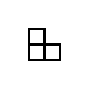
\begin{tikzpicture}[scale=0.2]
			\draw[thick] (0,0) rectangle (1,1);
			\draw[thick] (1,0) rectangle (2,1);
			\draw[thick] (0,1) rectangle (1,2);
			\end{tikzpicture}
			--shaped tiles.
			\end{theorem}

			\begin{solution}

			\end{solution}
		\end{questions}
	
\end{document}
